\begin{figure}[H]
    \centering
    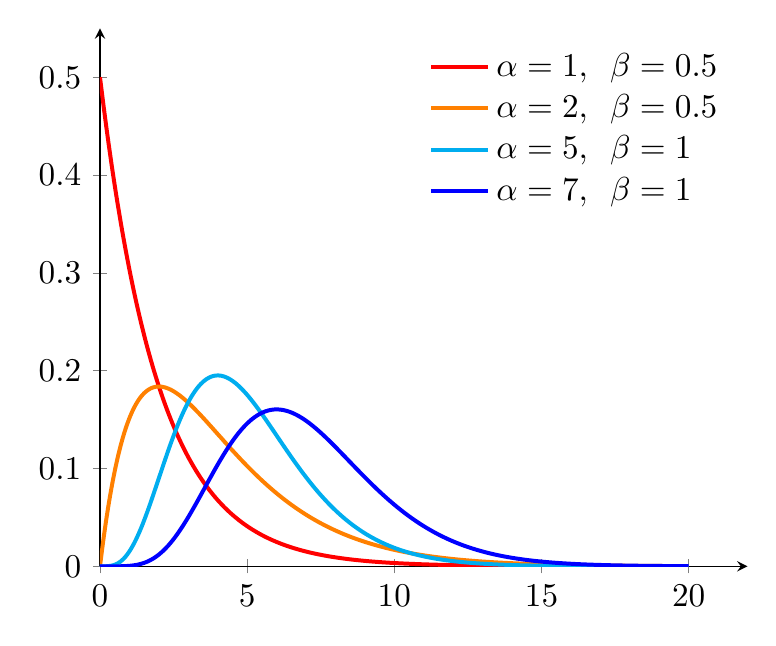
\begin{tikzpicture}[
        declare function={gamma(\z)= (2.506628274631*sqrt(1/\z) + 0.20888568*(1/\z)^(1.5) + 0.00870357*(1/\z)^(2.5) - (174.2106599*(1/\z)^(3.5))/25920 - (715.6423511*(1/\z)^(4.5))/1244160)*exp((-ln(1/\z)-1)*\z);},
        declare function={gammapdf(\x,\k,\theta) = \x^(\k-1)*exp(-\x/\theta) / (\theta^\k*gamma(\k));},
        scale=1.2
    ]
        \begin{axis}[
            axis lines = left,
            enlargelimits = upper,
            samples = 200,
            legend cell align = left,
            legend style = {draw=none}
        ]
            \addplot [smooth, domain=0:20, red, very thick] {gammapdf(x,1,2)};
            \addlegendentry{$\alpha=1,\hphantom{0} \beta=0.5$}
            \addplot [smooth, domain=0:20, orange, very thick] {gammapdf(x,2,2)};
            \addlegendentry{$\alpha=2,\hphantom{0} \beta=0.5$}
            \addplot [smooth, domain=0:20, cyan, very thick] {gammapdf(x,5,1)};
            \addlegendentry{$\alpha=5,\hphantom{0} \beta=1$}
            \addplot [smooth, domain=0:20, blue, very thick] {gammapdf(x,7,1)};
            \addlegendentry{$\alpha=7,\hphantom{0} \beta=1$}
        \end{axis}
    \end{tikzpicture}
\end{figure}